\subsection{Beta version}
\label{kap:McpExecutorBetaversion}
F�r die Betaversion der Mcp-Executor-Einheit werden alle Komponenten in ein Geh�use integriert (s. Abbildung \ref{fig:McpExecutorBeta}), welches gerade so gro� ist, dass es beim Tragen am K�rper m�glichst nicht st�rt und einfach befestigt werden kann. F�r das Integrieren werden zus�tliche Platinen angefertigt.
\newline
Aufgrund des Feststellens verschiedener negativer Aspekte w�hrend der Entstehung der Einheiten existieren mehrere Beta-Versionen, von denen jedoch nur die erste aufgeziegt wird.

\begin{figure}[H]
	\centering
	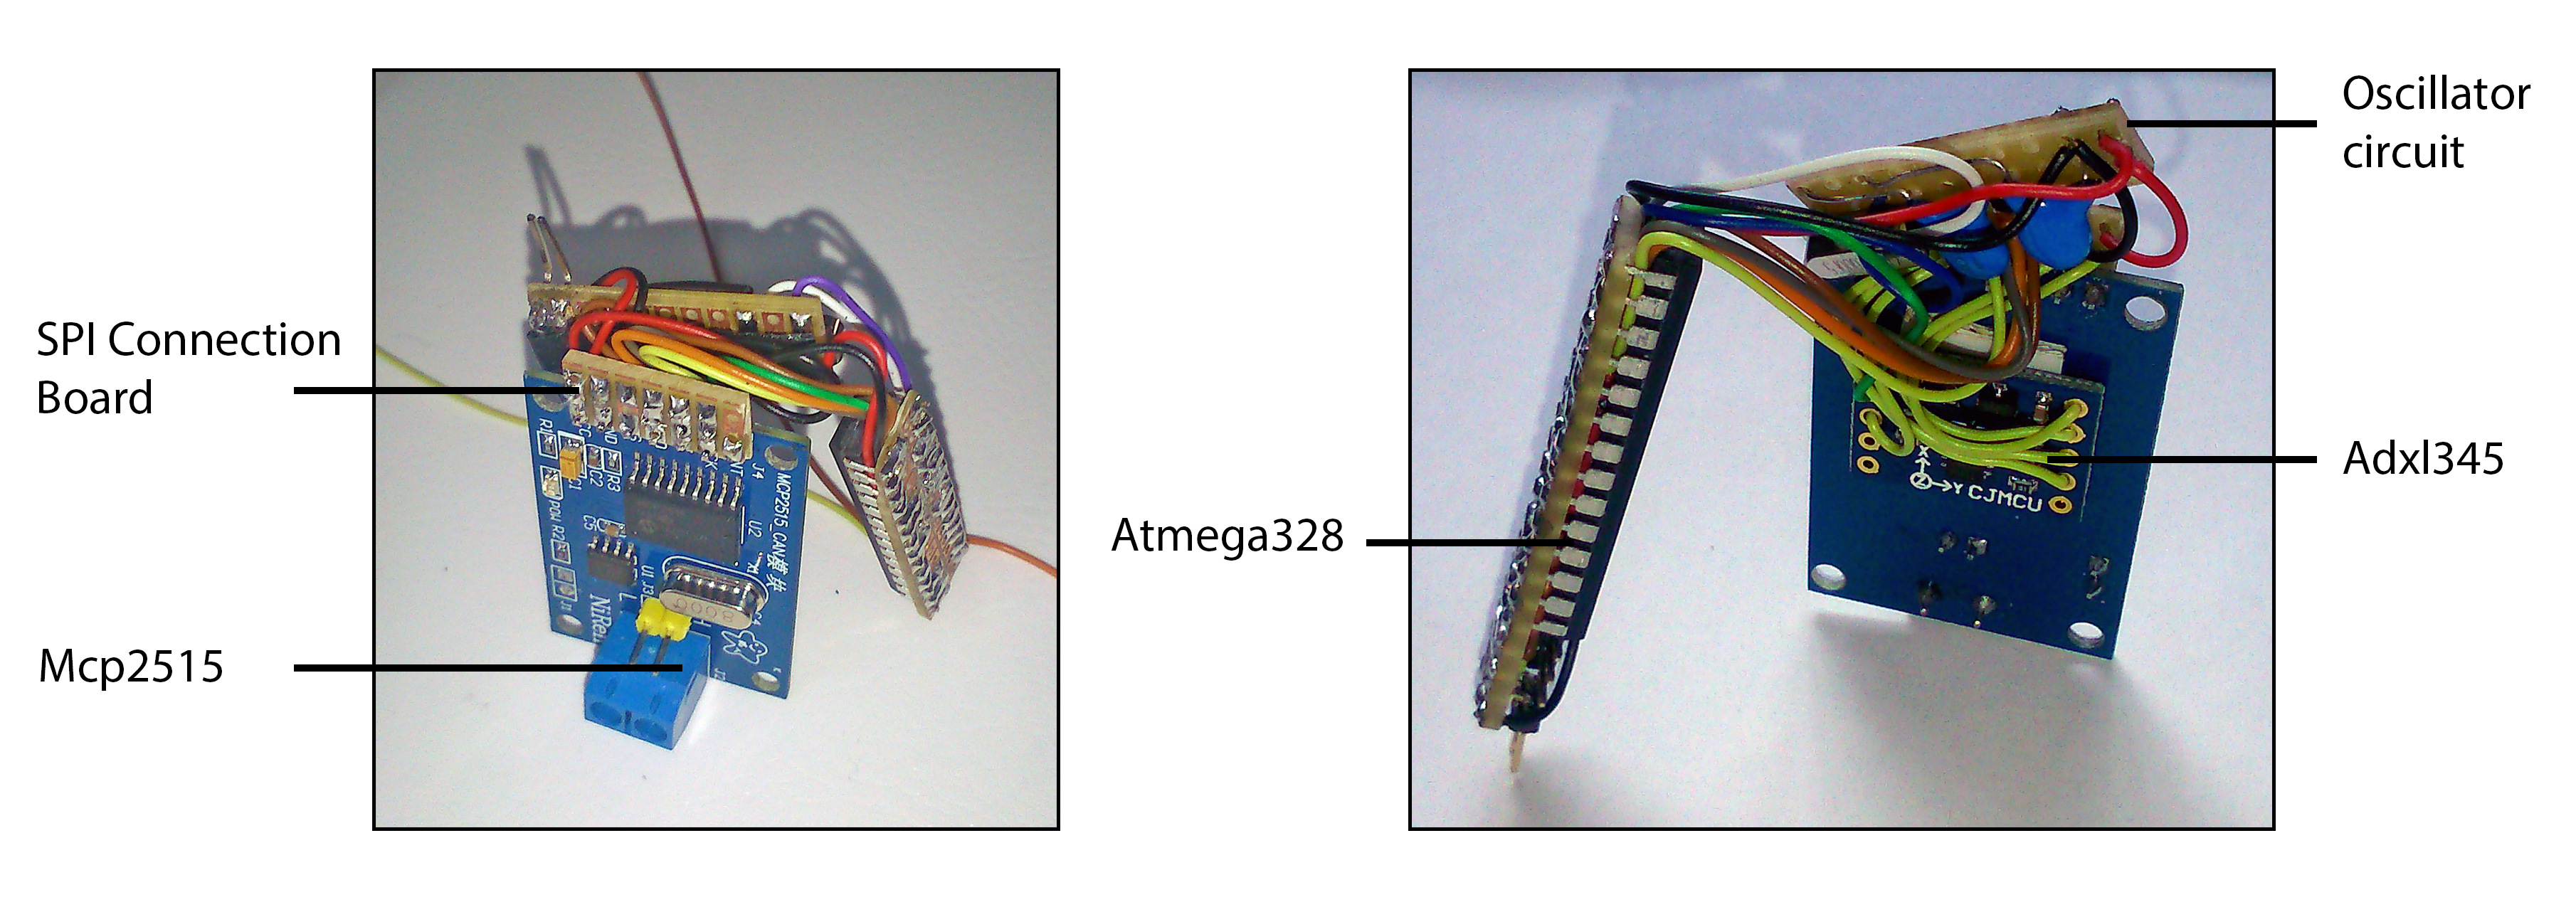
\includegraphics[width=1.0\linewidth]{03_Grafiken/Messsystem/McpExecutor_BetaDetail}
	\caption[Betaversion einer Mcp-Executor-Einheit]{Betaversion einer Mcp-Executor-Einheit}
	\label{fig:McpExecutorBeta}
\end{figure}

Die Befestigung der Einheit am K�rper erfolgt anhand eines Positioniergurtes. Dieser besteht in der ersten Beta-Version aus zwei und in der zweiten Version aus einem Klettverschluss, die an dem Abdeckblech der Einheit befestigt sind. Durch ein entsprechendes Gegenst�ck des Klettverschlusses auf der R�ckseite des Abdeckblechs ist der notwendig Halt gegeben.
%
% BILD KLETTVERSCHLUSS
%
\begin{figure}[H]
	\centering
	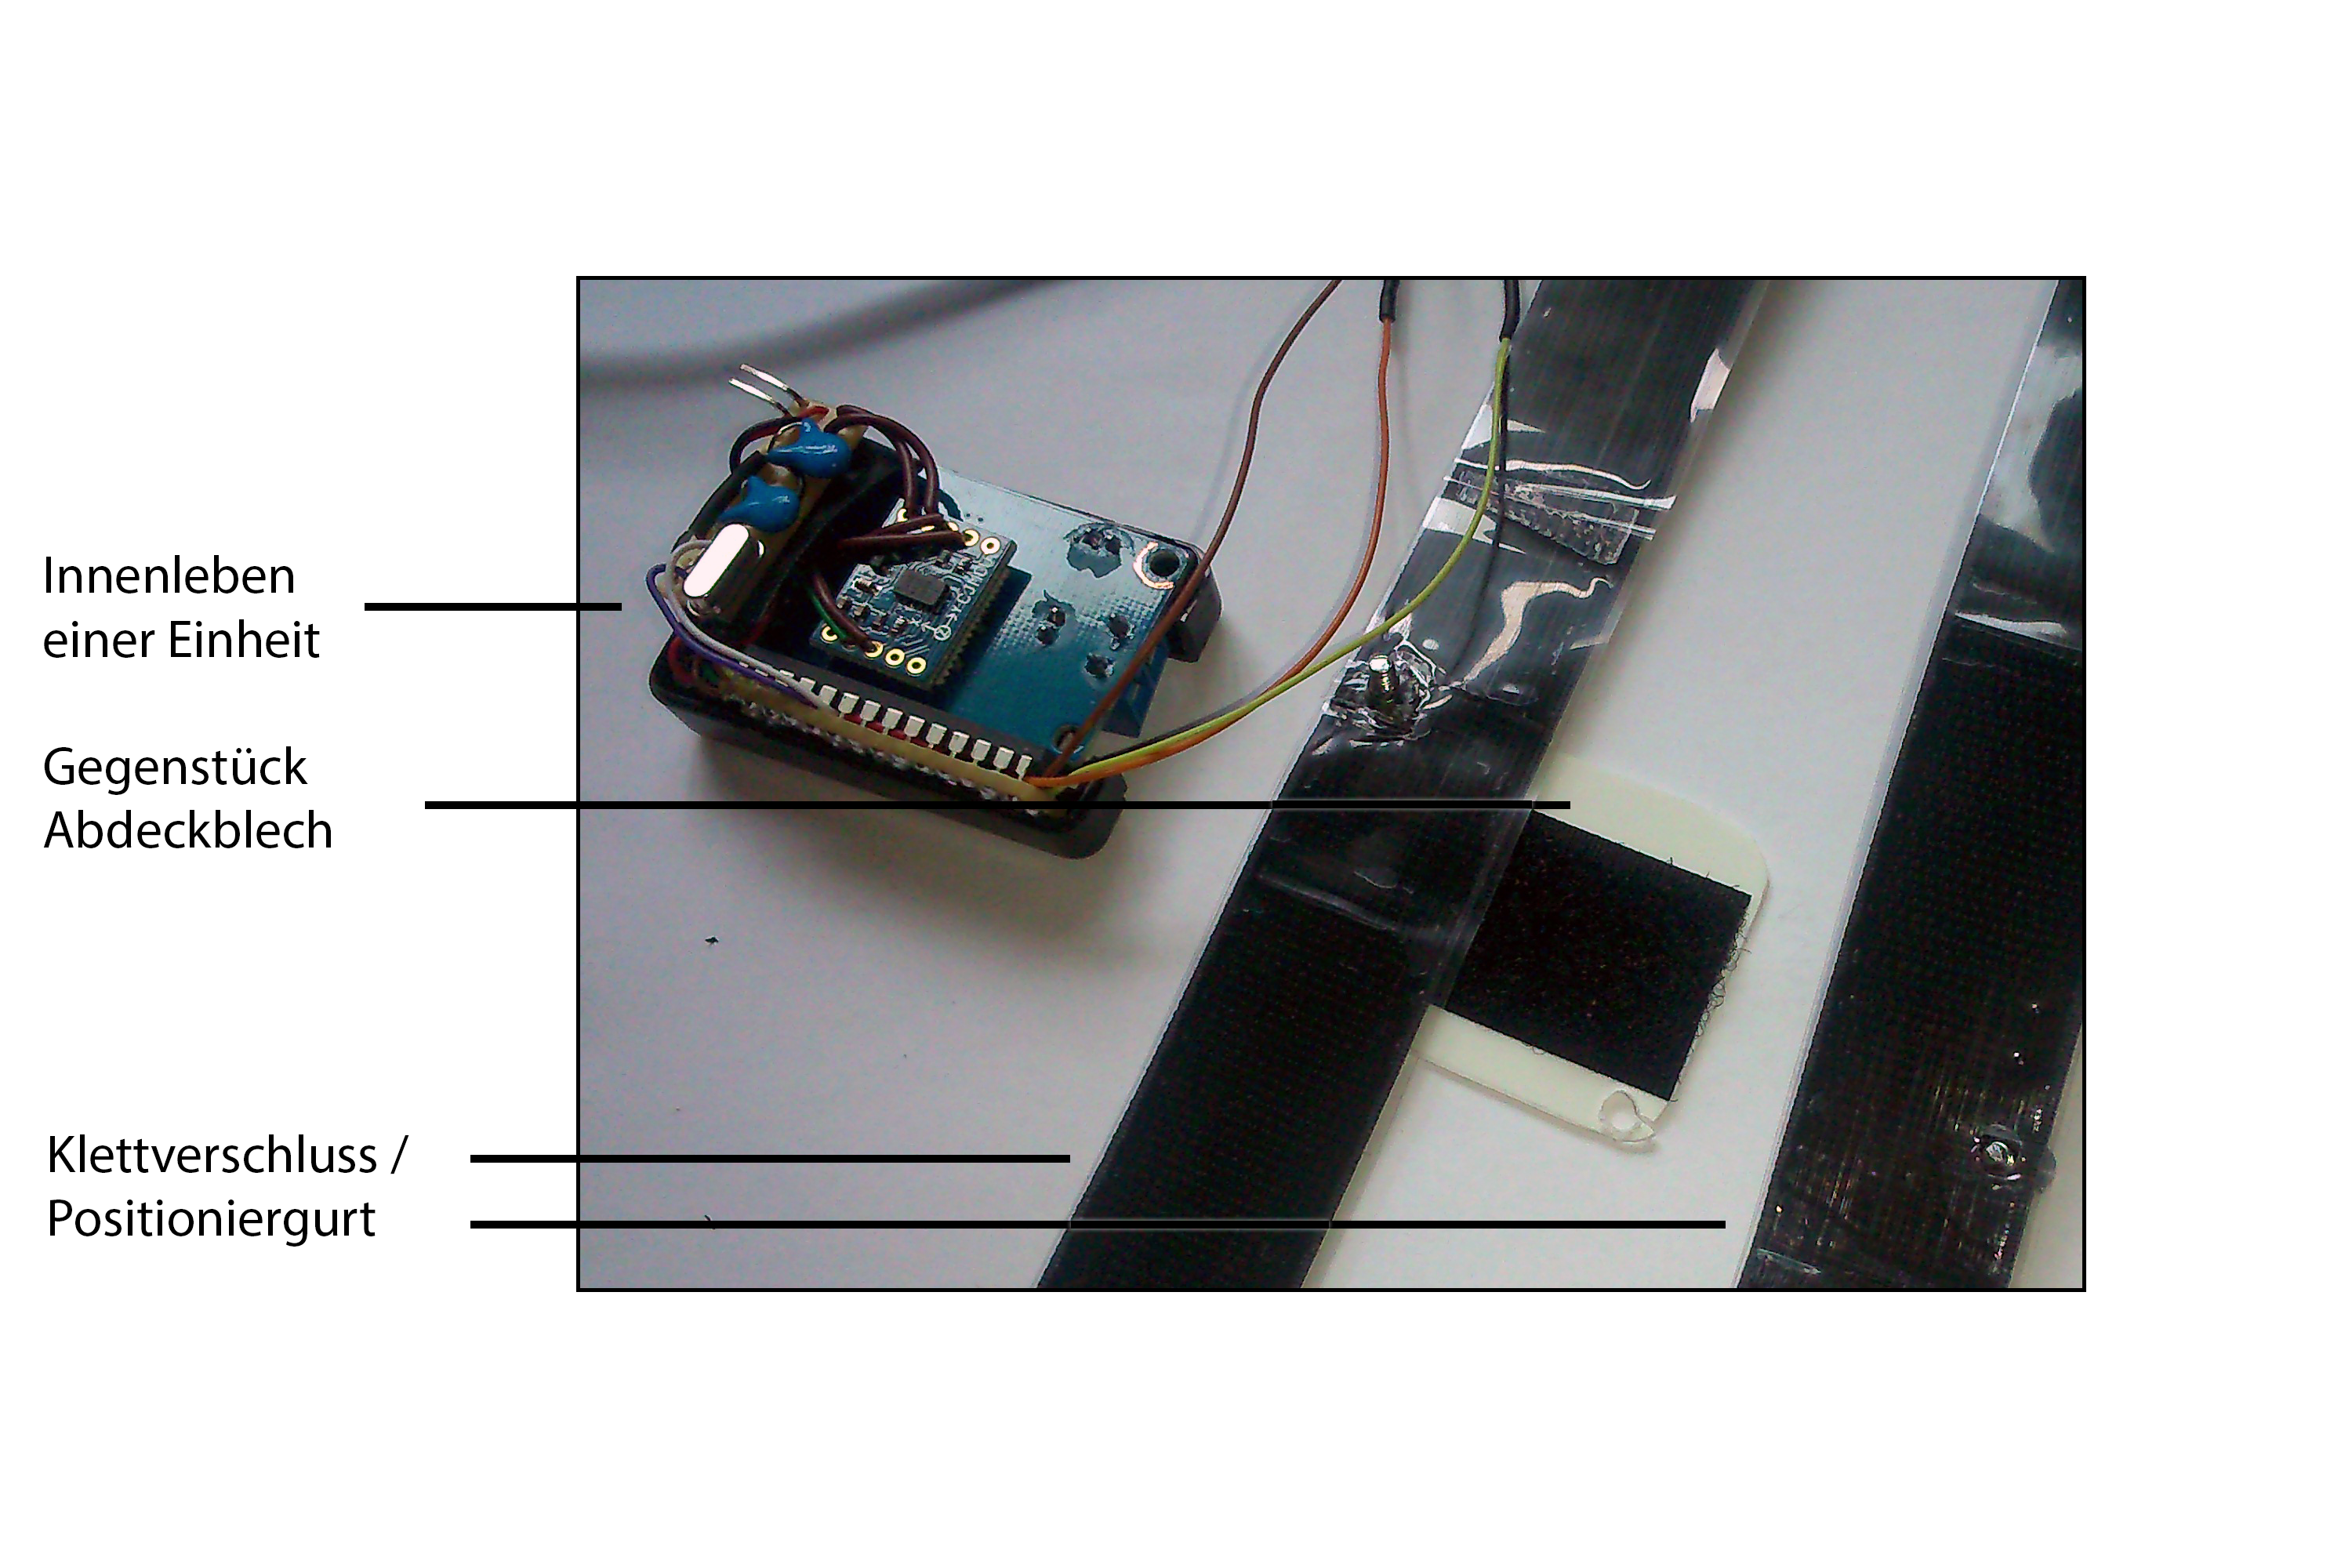
\includegraphics[width=1.0\linewidth]{03_Grafiken/Messsystem/McpExecutor2515Klettverschluss}
	\caption[Betaversion einer Mcp-Executor-Einheit - Klettverschluss]{Betaversion einer Mcp-Executor-Einheit - Klettverschluss}
	\label{fig:McpExecutorBetaKlettverschluss}
\end{figure}

An dem Anzug sind ebenfalls entsprechende Gegenst�cke des Klettverschlusses angebracht, sodass die Einheiten w�hrend der Bewegung nicht verrutschen. 

